\section{Actor-Critic}
\begin{frame}{}
    \LARGE Reinforcement Learning: \textbf{Actor-Critic}
\end{frame}

\begin{frame}{Actor-Critic}
    \begin{itemize}
        \item We do not know the true Q and V functions. Can we learn them?
        \pause
        \item Yes, by using Q-learning! We can combine Policy Gradients and Q-learning by training both an \textbf{actor} (the policy) and a \textbf{critic} (the value or Q-network).
        \pause
        \item The actor selects actions, while the critic evaluates how good the chosen actions are and provides feedback for improvement.
        \item The two networks adapt to each other, similar to the training process in GANs.
        \pause
        \item This approach simplifies the critic's task, as it only needs to estimate values for (state, action) pairs generated by the current policy.
        \item We can also incorporate Q-learning techniques, such as experience replay.
        \pause
        \item \textbf{Remark:} The advantage function measures how much better an action was compared to the expected value.
    \end{itemize}
\end{frame}

\begin{frame}{Actor-Critic Algorithm}
    \begin{figure}
        \centering
        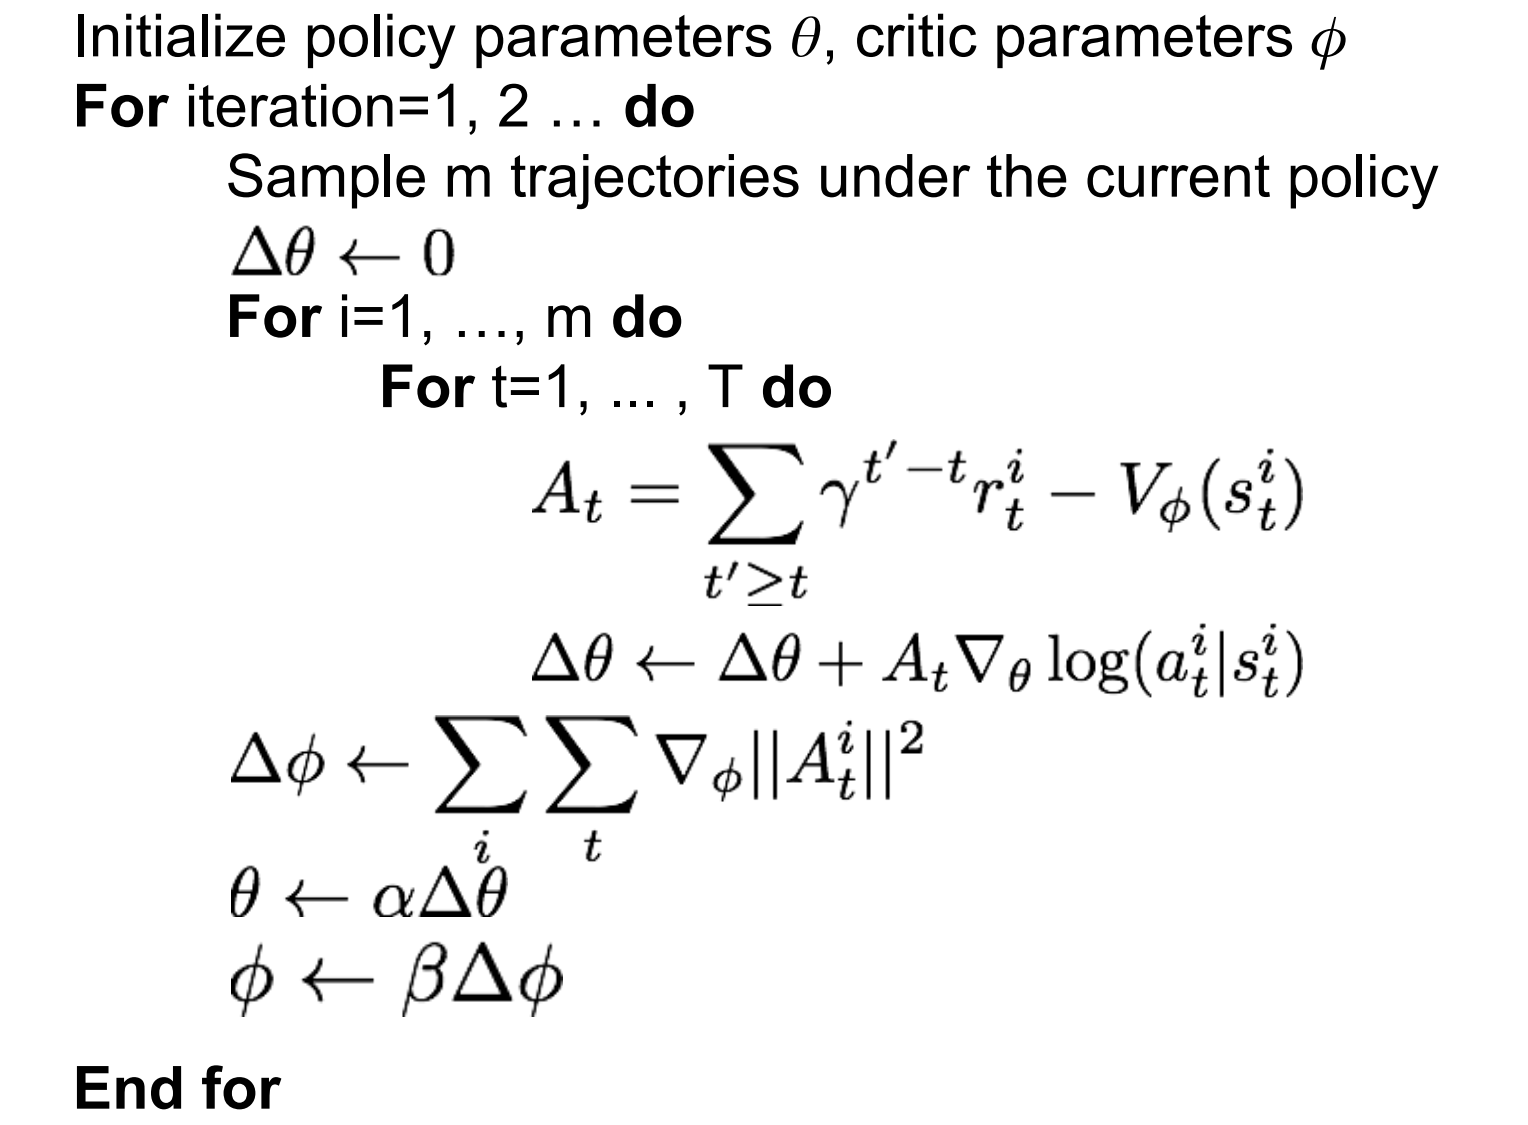
\includegraphics[width=0.9\textwidth,height=0.9\textheight,keepaspectratio]{images/policygrad+reinforce+actor/a2c.png}
    \end{figure}
\end{frame}
